\title{Decoders}
\begin{document}

\section{Binary Decoders}

\begin{frame}{Binary decoder}
  \begin{definition}
    A \alert{decoder} is a digital logic circuit that accepts $n$ inputs and $m$ outputs, where $n>m$.  Each input combination of the $n$ inputs corresponds to exactly one combination of the $m$ outputs.
  \end{definition}
  \begin{itemize}
    \item Usually, decoders are \alert{binary decoders}, which map $n$ inputs to $2^n$ outputs.
    \item So a 2 inputs binary decoder would have 4 outputs, and be called a 2-to-4 binary decoder.
  \end{itemize}
\end{frame}

\begin{frame}{2-to-4 Binary Decoder}
  Determine the truth table for the following 2-to-4 binary decoder.\\
  \begin{columns}
    \begin{column}{6cm}
      \begin{center}
        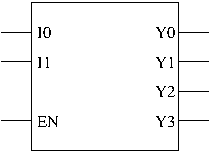
\includegraphics{2to4BinaryDecoderComponent}
      \end{center}
    \end{column}
    \begin{column}{6cm}
      \begin{center}
        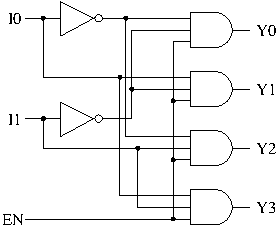
\includegraphics{2to4BinaryDecoderLogic}
      \end{center}
    \end{column}
  \end{columns}
\end{frame}

\section{74x138 Decoder}

\begin{frame}{74x138 decoder schematic diagram}
  \begin{center}
    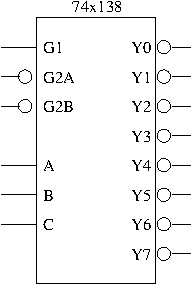
\includegraphics{74x138Schematic}
  \end{center}
\end{frame}

See page 388 of the text for the logic circuit.\\

Notice that $Y5\_L = (G1 \cdot G2A\_L' \cdot G2B\_L' \cdot C \cdot B' \cdot A)' = G1' + G2A\_L + G2B\_L + C' + B + A'$.

\section{Cascading Decoders}

\begin{frame}{The sky is the limit}
  \begin{block}{Key engineering principle}
    Break down a problem into simple parts, solve those parts, then use them to build a complex solution.
  \end{block}
  Using the relatively simple 74x138, we can build arbitrarily complex decoders.
  \begin{itemize}
    \item Page 391 of the text shows a 5-to-32 bit decoder.
    \item Notice how we can tie one of the inputs to a 74x138 low and create a 2-to-4 decoder.
    \item This decoder controls four other 74x138 decoders to completely decode th 5 bit input.
  \end{itemize}
\end{frame}

\section{Decoders in VHDL}

\begin{frame}{Decoders in VHDL}
  Let's look at an example of some decoder implementations in VHDL.
\end{frame}

\end{document}
